% GO TO: /Users/leonlufkin/Library/texmf/tex/latex
%        to add custom packages to the path
\documentclass{article}
\usepackage{report}

\title{Interpreting Dynamics}
\author{Leon Lufkin}
\date{\today}

\makeatletter
\let\Title\@title
\let\Author\@author
\let\Date\@date

\begin{document}

%%%%%%%%%%%%%
%% Setting %%
%%%%%%%%%%%%%
\section{Setting}
We can mostly explain symmetry breaking and tiling, and so we finally want to explain localization.
To do this, I focus on a single-neuron model with ReLU activation.

The task is to discriminate between two classes of inputs:
\begin{align}
  X_1 \sim p(\xi_1), \quad X_0 \sim p(\xi_0),
\end{align}
which are $n$-dimensional vectors.
We only assume that $p$ is \emph{translation-invariant} (this is explained more below) and that it is symmetric about 0, i.e. $p(x) = p(-x)$.
Inputs $X_i$ have scalar label $Y = i$, for $i = 0, 1$.
The distribution $p$ is paramaterized by $\xi > 0$, which defines the length-scale of correlations in the input.
Specifically, we construct $p$ so that
\begin{align}
  \operatorname{Cov}(X) = \Sigma(\xi), \quad \Sigma(\xi)_{ij} = k(i,j) \triangleq \exp(-(i-j)^2 / \xi^2).
\end{align}
Later, we will consider more general kernels $k$.

% \begin{figure}[!ht]
%   \centering
%   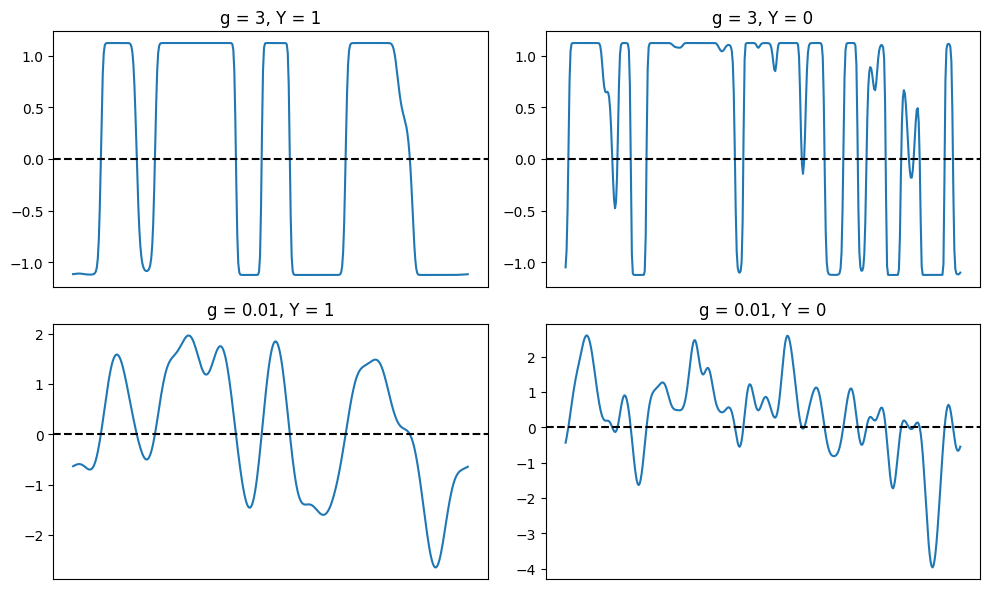
\includegraphics[width=0.7\textwidth]{figs/samples.png}
% \end{figure}

% We train a two-layer neural network on this task using gradient descent.
% \begin{align}
%   \hat{y}(x) = \frac{1}{K} \sum_{k=1}^{K} \sigma(\langle w_k, x \rangle + b_k),
% \end{align}
% \begin{figure}[!ht]
%   \centering
%   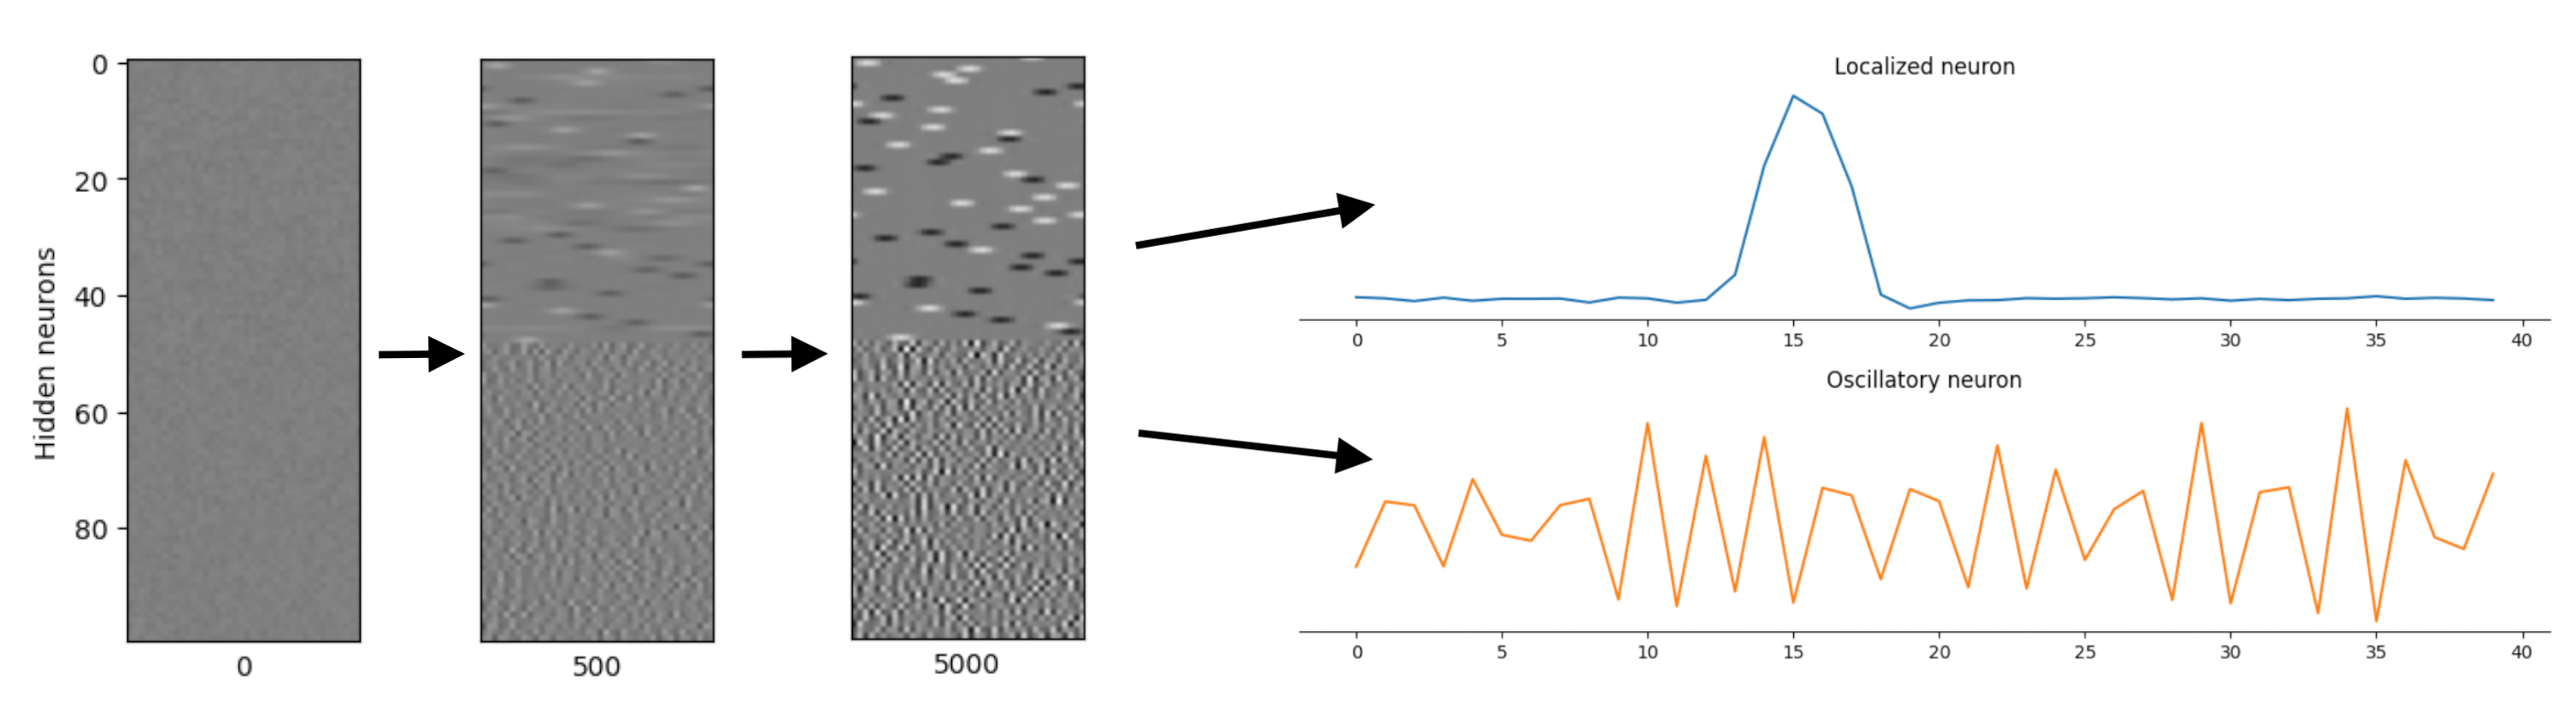
\includegraphics[width=\textwidth]{figs/fig_rfs_arrows.png}
% \end{figure}

We consider one neuron without bias and ReLU activation, since it's the simplest model that captures the localization phenomenon.
\begin{align}
  \hat{y}(x) = \operatorname{ReLU}(\langle w, x \rangle),
\end{align}
where $w$ is our receptive field.

%%%%%%%%%%%%%%
%% Dynamics %%
%%%%%%%%%%%%%%
\section{Dynamics}
The dynamics of $w$ is given by
\begin{align}
  \tau \frac{d}{dt} w
  &= - \frac{\partial \LL}{\partial w}
  % = \frac{1}{2} \underbrace{ \left[ \frac{\partial}{\partial w} \E_{ X \mid Y = Y_i } \left[ \operatorname{ReLU}(\langle w, x \rangle) \right] \right] }_{\triangleq f(w)} - \frac{1}{2} ( \Sigma_0 + \Sigma_1 ) w,
  = \frac{1}{2} \big[ \underbrace{ \E_{ X \mid Y = 1 } \left[ \mathbbm{1}(\langle w, X \rangle \geq 0) X \right] }_{\triangleq f(w)} \big] - \frac{1}{4} ( \Sigma_0 + \Sigma_1 ) w,
  \label{eq:dwdt}
\end{align}
% where $i$ is the class with output label 1, i.e. $Y_i = 1$ and $Y_{1-i} = 0$.
This elucidates some universal structure
% We could also write $f$ as
% \begin{align}
%   f(w) &= \E_{ X \mid Y = Y_i } \left[ \mathbbm{1}(\langle w, X \rangle \geq 0) X \right]. \label{eq:f}
% \end{align}
and lets us establish some properties of $f$.
\begin{enumerate}
  \item \emph{It is invariant to scaling $w$}: $f(w) = f(\alpha w)$ for $\alpha > 0$.
  \item \emph{It is sign equivariant}: $f(-w) = -f(w)$.
  \item \emph{It is translation equivariant\footnote{Here, ``translation'' refers to shifts of the \emph{entries} of a vector. So, if $\CC$ is a shift down by 1, $x_i = (\CC x)_{i+1}$}}: $f(\CC w) = \CC f(w)$, where $\CC$ is a circular shift.
\end{enumerate}
Thus, \underline{$f$ only depends on the shape of $w$, not it's magnitude or position}.
So, it is precisely the object we need to understand.
Note we can reduce properties 2 and 3 to the more general statement:
\begin{enumerate}
  \item[4.] \emph{It can preserve symmetry in $p$}: If $p$ is symmetric w.r.t. some invertible linear  transformation $A$, i.e. $p_{\xi}(x) = p_{\xi}(A x)$ for all $x$, then $f(A w) = A^{-\top} f(w)$.
  If $A$ is orthogonal, then $f(A w) = A f(w)$.
\end{enumerate}

% The above equation also makes precise why a Gaussian approximation empirically always holds early in training.
% Early on, with $w$ initialized as standard Gaussian, the second term dominates the dynamics.
% Note this term looks a lot like the update rule if we assume $p$ is Gaussian.

% \subsection{Interpretation}
% How can we understand what \cref{eq:dwdt} is doing?
% We focus on the second term, $(\Sigma_0 + \Sigma_1) w$, first, since $f$ will take more work to understand.
What is the second term, $(\Sigma_0 + \Sigma_1) w$, doing?
It's immediately clear that it is a \emph{shrinkage term} since $\Sigma$ is positive semi-definite.
% It shrinks the receptive field, specifically shrinking lower-frequency oscillations faster than higher-frequency ones\footnote{Does this make sense?}.
% Once $w$ becomes sufficiently small in norm so that the second term is on the order of $f(w)$, the first term is no longer negligible, and the dynamics are no longer Gaussian.


% It can be understood in terms of: (1) smoothing, and (2) frequencies. 
One could try to understand in terms of the convolutions implemented by $\Sigma_0$ and $\Sigma_1$, which we call $k_0$ and $k_1$, respectively\footnote{Recall $\Sigma$ is circulant.}. 
% The first interpretation comes directly from how we define $\Sigma$.
% The covariance between any two points is given by some translation-invariant kernel $k(x,y)$.
% So, each row in $\Sigma$ is identical, except that the density for the $i$-th row is peaked at column $i$.
So, we can write the second term as $(k_0 + k_1) * w$.
However, I still find it hard to understand how this drives the dynamics.
\emph{I could use some help here.}

Another way to interpret the second term is by using the discrete Fourier transform.
Because $\Sigma_0$ and $\Sigma_1$ are circulant matrices, they both diagonalize in the discrete Fourier basis\footnote{In particular, we can take the real and imaginary parts of the complex Fourier modes because $\Sigma$ is always real and symmetric.}, which we denote $P$.
Let $\Lambda_i$ be the diagonal matrix of eigenvalues for $\Sigma_i$.
Representing $w$ in Fourier space by $u = P^\top w$, we have
\begin{align}
  \tau \frac{d}{dt} u
  &= \frac{1}{2} P^\top f(P u) - \frac{1}{2} ( \Lambda_0 + \Lambda_1 ) u.
  \label{eq:dudt}
\end{align}
Note the eigenvalues in $\Lambda_0$ and $\Lambda_1$ are all positive, but $\Lambda_1$ weights lower-frequency oscillations more heavily than $\Lambda_0$, and higher-frequency ones less.
Together, they act to shrink low-frequency oscillations faster than high-frequency ones\footnote{Shouldn't it be the other way around?}.

\paragraph*{Extra fact}
One additional thing we can say about $f$ is that
\begin{align*}
  \frac{\partial}{\partial w} f(w)_i \perp w \quad \forall i,
  \qquad \text{and} \qquad
  \frac{\partial}{\partial w_j} f(w) \perp w \quad \forall j.
\end{align*}
This is either something important about interpreting $f$ or entirely obvious.
Not sure which, but this seems like a special consequence of using ReLU activation.
To see why:
\begin{align*}
  \frac{\partial}{\partial w_j} f(w)_i
  &= \frac{\partial}{\partial w_j} \int_{\R^n} p_{\xi}(x) \mathbbm{1}(\langle w, x \rangle \geq 0) x_i dx
  = \int_{\R^n} p_{\xi}(x) \delta(\langle w, x \rangle) x_i x_j dx,
\end{align*}
where $\delta$ is the Dirac delta function.

\subsection{General Setting}
We isolate the $i$-th entry,% and ignore our dependence on $Y=1$,
\begin{align*}
  f(w)_i
  &= \E_{X \mid Y = 1} \left[ \mathbbm{1}(\langle w, X \rangle \geq 0) X_i \right] \\
  &= \E_{X_i \mid Y = 1} \left[ X_i \E_{ X \mid Y = 1, X_i } \left[ \mathbbm{1}(\langle w, X \rangle \geq 0) \right] \right] \\
  &= \E_{X_i \mid Y = 1} \left[ X_i \Pr\left( \langle w, X \rangle \geq 0 \mid Y = 1, X_i \right) \right].
\end{align*}
Let's focus on the probability term, starting by writing all the randomness on the left side:
\begin{align*}
  \Pr\left( \langle w, X \rangle \geq 0 \mid Y = 1, X_i \right)
  % &= \Pr\left( \sum_{k=1}^{n} w_k X_k \geq 0 \mid Y = Y_i, X_j \right) \\
  &= \Pr\left( \sum_{j \neq i} w_j X_j \geq -w_i X_i \mid Y = 1, X_i \right).
\end{align*}
This probability is impossible to compute exactly in general, but we can use a Gaussian approximation on $X \mid Y = 1, X_i$ to make it tractable.
Let $\mu_{\mid X_i}$ $\Sigma_{\mid X_i}$ be the mean and covariance for $X_{\not i} \mid Y = 1, X_i \in \R^{n-1}$, where $X_{\not i}$ is the vector $X$ with the $i$-th entry removed.
Then, $\sum_{j \neq i} w_j X_j \mid Y = 1, X_i \sim \NN(w_{\not i}^\top \mu_{\mid X_i}, w_{\not i}^\top \Sigma_{\mid X_i} w_{\not i})$.
So,
\begin{align*}
  \Pr\left( \langle w, X \rangle \geq 0 \mid Y = 1, X_i \right)
  &\approx 1 - \Phi\left( \frac{ -w_i X_i - w_{\not i}^\top \mu_{\mid X_i} }{ \sqrt{ w_{\not i}^\top \Sigma_{\mid X_i} w_{\not i} } } \right)
  = \Phi\left( \frac{ w_i X_i + w_{\not i}^\top \mu_{\mid X_i} }{ \sqrt{ w_{\not i}^\top \Sigma_{\mid X_i} w_{\not i} } } \right).
\end{align*}
% We can simplify this by redefining $\mu_{i \mid X_j}$ and $\Sigma_{i \mid X_j}$ to include $X_j$.
% Because we are conditioning on $X_j$, the corresponding mean and variance are $X_j$ and 0, respectively.
% So, if we adjust the other entries of $\mu_{i \mid X_j}$ and $\Sigma_{i \mid X_j}$ to account for this, we get
% \begin{align*}
%   \Pr\left( \langle w, X \rangle \geq 0 \mid Y = Y_i, X_j \right)
%   &\approx \Phi\left( \frac{ w^\top \mu_{i \mid X_j} }{ \sqrt{ w^\top \Sigma_{i \mid X_j} w} } \right).
% \end{align*}
Thus,
\begin{align}
  f(w)_i &\approx \E_{X_i \mid Y=1} \left[ X_i \Phi\left( \frac{ w_i X_i + w_{\not i}^\top \mu_{\mid X_i} }{ \sqrt{ w_{\not i}^\top \Sigma_{\mid X_i} w_{\not i} } } \right) \right]. \label{eq:fwi_seperated}
\end{align}

\paragraph*{Rewriting}
Finally, let us rewrite this a bit to highlight its similarity to the Gaussian case.
Let us define $\tilde{\mu}_{\mid X_i}$ and $\tilde{\Sigma}_{\mid X_i}$ to be the mean and covariance for $X \mid Y = 1, X_i \in \R^n$.
Note the $i$-th entry of $\tilde{\mu}_{\mid X_i}$ is $X_i$ and the $j$-th row and column of $\tilde{\Sigma}_{\mid X_i}$ are 0.
Then, $w_i X_i + w_{\not i}^\top \mu_{\mid X_i} = w^\top \tilde{\mu}_{\mid X_i}$ and $w_{\not i}^\top \Sigma_{\mid X_i} w_{\not i} = w^\top \tilde{\Sigma}_{\mid X_i} w$.
So,
\begin{align}
  f(w)_i 
  &\approx \E_{X_i \mid Y=1} \left[ X_i \Phi\left( \frac{ w^\top \tilde{\mu}_{\mid X_i} }{ \sqrt{ w^\top \tilde{\Sigma}_{\mid X_i} w } } \right) \right] \label{eq:fwi_collapsed} \\
  % &= \E_{X_i \mid Y=1} \left[ X_i \Phi\left( \frac{ w^\top \tilde{\mu}_{\mid X_i} }{ \sqrt{ w^\top ( \E_{X \mid X_i, Y=1} \left[ X X^\top \right] - \tilde{\mu}_{\mid X_i} \tilde{\mu}_{\mid X_i}^\top ) w } } \right) \right] \\
  &= \E_{X_i \mid Y=1} \left[ X_i \Phi\left( \frac{ w^\top \tilde{\mu}_{\mid X_i} }{ \sqrt{ \E_{X \mid X_i, Y=1} \left[ (w^\top X)^2 \right] - (w^\top \tilde{\mu}_{\mid X_i})^2 } } \right) \right]
\end{align}
% Let us further rewrite the conditional covariance:
% \begin{align*}
%   \tilde{\Sigma}_{\mid X_i}
%   % &= \E_{X \mid X_i, Y=1} \left[ X X^\top \right] - (\E_{X \mid X_i, Y=1} \left[ X \right]) (\E_{X \mid X_i, Y=1} \left[ X \right])^\top
%   &= \E_{X \mid X_i, Y=1} \left[ X X^\top \right] - \tilde{\mu}_{\mid X_i} \tilde{\mu}_{\mid X_i}^\top.
% \end{align*}
What can we say about the conditional mean?
We can relate it to the unconditional covariance:
\begin{align*}
  [(\Sigma_1)_{ji} ]_{j\in[n]}
  &= \E_{X \mid Y=1} \left[ X_i X \right]
  = \E_{X_i \mid Y=1} \left[ X_i \E_{X \mid X_i, Y=1} \left[ X \right] \right]
  = \E_{X_i \mid Y=1} \left[ X_i \tilde{\mu}_{\mid X_i} \right]
  = \E_{X_i \mid X_i > 0, Y=1} \left[ X_i \tilde{\mu}_{\mid X_i} \right],
\end{align*}
where last step follows by the symmetry of $p$ about 0, and the term on the left is the $i$-th column of $\Sigma_1$.

Note that $(\tilde{\mu}_{\mid X_i})_i = X_i$ (duh).
Because all the entries are symmetric about 0, we'd expect that $(\tilde{\mu}_{\mid X_i})_j \leq X_i$ for $j \neq i$.
In particular, we'd expect that $(\tilde{\mu}_{\mid X_i})_j \approx 0$ for $j$ such that the $k_i(j) \approx 0$, i.e. they are uncorrelated.
Of course, this is not true in general, uncorrelatedness need not imply independence, but when is it sorta true?
In fact, this is not true in the single-pulse case, where far apart points can be anti-correlated.



% \begin{align*}
%   0
%   &\overset{?}{=} \E_{X \mid Y=1} \left[ X_i X X^\top \right]
%   = \E_{X_i \mid Y=1} \left[ X_i \E_{X \mid X_i, Y=1} \left[ X X^\top \right] \right] \\
%   &= \E_{X_i \mid Y=1} \left[ X_i \left( \tilde{\Sigma}_{\mid X_i} + \tilde{\mu}_{\mid X_i} \tilde{\mu}_{\mid X_i}^\top \right) \right]
%   = \E_{X_i \mid Y=1} \left[ X_i \tilde{\Sigma}_{\mid X_i} \right] + \E_{X_i \mid Y=1} \left[ X_i \tilde{\mu}_{\mid X_i} \tilde{\mu}_{\mid X_i}^\top \right] \\
%   &= \E_{X_i \mid Y=1} \left[ X_i \tilde{\Sigma}_{\mid X_i} \right] + \E_{X_i \mid Y=1} \left[ [(\Sigma_1)_{ij} ]_{j\in[n]} \tilde{\mu}_{\mid X_i}^\top \right] \\
%   &= \E_{X_i \mid Y=1} \left[ X_i \tilde{\Sigma}_{\mid X_i} \right] 
% \end{align*}
We can also relate the conditional and unconditional covariances.
Note,
\begin{align*}
  \Sigma_1
  &= \E_{X \mid Y=1} \left[ X X^\top \right] 
  = \E_{X_i \mid Y=1} \left[ \E_{X \mid X_i, Y=1} \left[ X X^\top \right] \right] 
  = \E_{X_i \mid Y=1} \left[ \tilde{\Sigma}_{\mid X_i} + \tilde{\mu}_{\mid X_i} \tilde{\mu}_{\mid X_i}^\top \right],
  % &= \E_{X_i \mid X_i>0, Y=1} \left[ \tilde{\Sigma}_{\mid X_i} \right].
\end{align*}
so,
\begin{align*}
  \E_{X_i \mid Y=1} \left[ \tilde{\Sigma}_{\mid X_i} \right]
  &= \Sigma_1 - \E_{X_i \mid Y=1} \left[ \tilde{\mu}_{\mid X_i} \tilde{\mu}_{\mid X_i}^\top \right].
\end{align*}
I don't know how much more we can say about $\tilde{\mu}_{\mid X_i}$ or $\tilde{\Sigma}_{\mid X_i}$ in general.

\subsection{Gaussian Data}
For Gaussian data, we can evaluate $f(w)$ exactly.
Using simpler analytical methods, we get,
\begin{align}
  f(w) &= \frac{1}{\sqrt{2\pi}} \cdot \frac{ \Sigma_1 w }{ \sqrt{w^\top \Sigma_1 w} }. \label{eq:f_gaussian}
\end{align}
But how do we arrive at this result from our expression for $f(w)_i$ above, and does this elucidate why localization does not occur for Gaussian data?
Starting from \cref{eq:fwi_seperated}, we have
\begin{align*}
  f(w)_i &= \frac{1}{2} \int_{\R} \frac{1}{\sqrt{2\pi}} e^{-\frac{1}{2} x_i^2} \left[ x_i \operatorname{erf}\left( \frac{ w_i x_i + w_{\not i}^\top \mu_{\mid X_i=x_i} }{ \sqrt{ 2 w_{\not i}^\top \Sigma_{\mid X_i=x_i} w_{\not i} } } \right) \right] dx_i.
\end{align*}
We need to express $\mu_{\mid X_i=x_i}$ and $\Sigma_{\mid X_i=x_i}$ in terms of $x_i$.
Note that
\begin{align*}
  \mu_{\mid X_i=x_i}
  &= \begin{bmatrix} (\Sigma_1)_{ij} \end{bmatrix}_{j \neq i} x_i,
\end{align*}
and
\begin{align*}
  \Sigma_{\mid X_i=x_i}
  &= \begin{bmatrix} (\Sigma_1)_{kj} \end{bmatrix}_{k,j \neq i} - \begin{bmatrix} (\Sigma_1)_{ij} \end{bmatrix}_{j \neq i} \begin{bmatrix} (\Sigma_1)_{ij} \end{bmatrix}_{j \neq i}^\top.
\end{align*}
Importantly, this is independent of $x_i$.
Note that we can write $w_i x_i + w_{\not i}^\top \mu_{\mid X_i=x_i} = w^\top \begin{bmatrix} (\Sigma_1)_{ij} \end{bmatrix}_{j\in[n]} x_i$ (we noted this for the general case above as well).
We will denote $\begin{bmatrix} (\Sigma_1)_{ij} \end{bmatrix}_{j\in[n]}$ by $k_i$.
So,
\begin{align*}
  f(w)_i 
  &= \frac{1}{2} \int_{\R} \frac{1}{\sqrt{2\pi}} e^{-\frac{1}{2} x_i^2} \Bigg[ x_i \operatorname{erf}\Bigg( \underbrace{ \frac{ k_i^\top w }{ \sqrt{ 2 w_{\not i}^\top \Sigma_{\mid X_i=x_i} w_{\not i} } } }_{\triangleq a} x_i \Bigg) \Bigg] dx_i \\
  &= \frac{1}{\sqrt{2\pi}} \int_0^\infty e^{- b^2 x_i^2} \left[ x_i \operatorname{erf}\left( a x_i \right) \right] dx_i && \text{where } b = \frac{1}{\sqrt{2}} \\
  &= \frac{1}{\sqrt{2\pi}} \frac{a}{2b^2} ( a^2 + b^2 )^{-\frac{1}{2}} && \text{via Ng \& Geller (1968)} \\
  % &= \frac{1}{\sqrt{2\pi}} \frac{a}{\sqrt{a^2+b^2}} \\
  % &= \frac{1}{\sqrt{2\pi}} \frac{1}{2b^2} \frac{ \frac{ k_i^\top w }{ \sqrt{ w_{\not i}^\top \Sigma_{\mid X_i=x_i} w_{\not i} } } }{ \sqrt{ \frac{ (k_i^\top w)^2 }{ w_{\not i}^\top \Sigma_{\mid X_i=x_i} w_{\not i} } + 2b^2 } } \\
  &= \frac{1}{\sqrt{2\pi}} \frac{1}{2b^2} \frac{ k_i^\top w }{ \sqrt{ (k_i^\top w)^2 + 2b^2 w_{\not i}^\top \Sigma_{\mid X_i=x_i} w_{\not i} } } \\
  % &= \frac{1}{\sqrt{2\pi}} \frac{1}{2b^2} \frac{ k_i^\top w }{ \sqrt{ 2b^2 w^\top \Sigma_1 w - (2b^2-1) (k_i^\top w)^2 } } \\
  &= \frac{1}{\sqrt{2\pi}} \frac{1}{(2b^2)^{\frac{3}{2}}} \frac{ k_i^\top w }{ \sqrt{ w^\top \Sigma_1 w - ( 1 - \frac{1}{2b^2} ) (k_i^\top w)^2 } }.
\end{align*}
Plugging in $b$,
\begin{align*}
  f(w)_i 
  % &= \frac{1}{\sqrt{2\pi}} \frac{ k_i^\top w }{ \sqrt{ (k_i^\top w)^2 + w_{\not i}^\top \Sigma_{\mid X_i=x_i} w_{\not i} } } \\
  &= \frac{1}{\sqrt{2\pi}} \frac{ k_i^\top w }{ \sqrt{ w^\top \Sigma_1 w } },
\end{align*}
precisely as desired.
The scaling term here \emph{no longer depends on $k_i$}, which is what drives localization for the high-gain case.
This happened because of the $b$ term in the denominator, which corresponds to the inverse of the standard deviation of the Gaussian distribution.
Could we tinker with $b$ and still get localization?
We would need to make $b$ large, which would require decreasing the variance of the Gaussian.
If we scale $\Sigma_1$, the covariance of $X$, to $\alpha \Sigma_1$, then $b^{-2}$ would scale to $\alpha b^{-2}$.
Importantly, $(k_i^\top w)^2$ would scale to $\alpha^2 (k_i^\top w)^2$.
So, after scaling by $\alpha$, we get 
\begin{align*}
  f(w)_i 
  &= \frac{1}{\sqrt{2\pi}} \frac{\sqrt{\alpha}}{(2b^2)^{\frac{3}{2}}} \frac{ k_i^\top w }{ \sqrt{ w^\top \Sigma_1 w - \alpha ( 1 - \frac{\alpha}{2b^2} ) (k_i^\top w)^2 } }.
\end{align*}
As $\alpha \to 0$, the localization term still disappears because of the extra power of $\alpha$ we pick up from $k_i$ being squared. 
Thus, scaling down the variance still will not yield localization.
Making $\alpha$ larger also won't yield localization, albeit differently.
In this case, the $(k_i^\top w)^2$ dominates, but it does not have a negative sign, so as $w$ gets more localized, $f(w)_i$ decreases, thus actively working against localization.
(Also, the integral's expression is only valid when $|b| > |a|$, so messing with $\alpha$ too much will break this.)


\subsection{Elliptical Data}
We cannot solve $f(w)$ exactly for most distributions, but for data from an elliptical distribution, we can at least give $f$ enough structure to understand its behavior.
An elliptical distribution $\operatorname{El}(\mu, \Sigma, \psi)$ has characteristic function $\phi_{X-\mu}(t) = \psi(t^\top \Sigma t)$.
This gives the property that if $X \sim \operatorname{El}(\mu, \Sigma, \psi)$, then $c + A X \sim \operatorname{El}(c + A \mu, A \Sigma A^\top, \psi)$.
We can use this to conclude that $\langle w, X \rangle \sim \operatorname{El}(\langle w, \mu \rangle, w^\top \Sigma w, \psi)$.
We can write the density of $S = \langle w, X \rangle$ as
\begin{align*}
  p(s) &= k \cdot g\left( \frac{s^2}{w^\top \Sigma w} \right),
\end{align*}
where $k$ is a normalizing constant.
Then,
\begin{align*}
  \E_X\left[ \operatorname{ReLU}(\langle w, X \rangle) \right]
  &= \E_S\left[ \operatorname{ReLU}(S) \right]
  = \int_0^{\infty} s p(s) ds
  = k \int_{0}^{\infty} s g\left( \frac{s^2}{w^\top \Sigma w} \right) ds.
\end{align*}
So,
\begin{align*}
  f(w)
  &= \frac{\partial}{\partial w} \left[ \E_X\left[ \operatorname{ReLU}(\langle w, X \rangle) \right] \right]
  = 2 k \int_{0}^{\infty} s \frac{\partial}{\partial w} \left[ g\left( \frac{s^2}{w^\top \Sigma w} \right) \right] ds \\
  &= -2 k \left[ \int_{0}^{\infty} s^3 g'\left( \frac{s^2}{w^\top \Sigma w} \right) ds \right] \frac{\Sigma w}{(w^\top \Sigma w)^2}.
\end{align*}
Setting $s = (\sqrt{w^\top \Sigma w}) u$, we have $ds = (\sqrt{w^\top \Sigma w}) du$, so
\begin{align*}
  f(w)
  &= -2 k \left[ \int_{0}^{\infty} u^3 (\sqrt{w^\top \Sigma w})^3 g'\left( u^2 \right) du \right] \frac{\Sigma w}{(w^\top \Sigma w)^2}
  \propto \frac{ \Sigma w }{ \sqrt{w^\top \Sigma w} },
\end{align*}
which is similar in form to the Gaussian case.
Given this form, we can write the update in Fourier space, given by $u = P^\top w$, where $P$ is the (real) DFT matrix.
\begin{align}
  \tau \frac{d}{dt} u
  &= \frac{c}{2} \frac{ \Lambda_1 u }{ \sqrt{ u^\top \Lambda_1 u } } - \frac{1}{4} ( \Lambda_0 + \Lambda_1 ) u,
\end{align}
where the $\Lambda_i$ are diagonal matrices of eigenvalues of $\Sigma_i$.
Because this is diagonal, we can compute steady states, which lets us show that the limiting solutions are a superposition of just one or two modes (i.e. $u$ is sparse)\footnote{I need to confirm this with simulations.}.
This is insufficient for localization, which requires $u$ to be sparse in the \emph{spatial} domain, not the Fourier domain.

How can we connect this to the representation in \cref{eq:fwi_collapsed}, and reconcile it with the apparent observation that marginal support on $\{ \pm 1 \}$ is sufficient for localization?
Let us consider an elliptical distribution with marginal that has support on $\{ \pm 1 \}$.
% I don't think it's possible to construct an elliptical distribution with a \emph{marginal} that has mass far from 0.
This would be achieved by $g(x) = \mathbbm{1}(x = 1)$. 
Then, $[(\Sigma_1)_{ji}]_{j\in[n]} = \tilde{\mu}_{\mid X_i = 1}$ and $\tilde{\Sigma}_{\mid X_i = 1} = \Sigma_1 - \tilde{\mu}_{\mid X_i = 1} \tilde{\mu}_{\mid X_i = 1}^\top$.
So, we just need to understand what $\Sigma_1$, the covariance, looks like as a function of $\Sigma$, the shape parameter (which need not be the covariance).
\begin{align*}
  (\Sigma_1)_{ij} 
  &= \E_{X} \left[ X_i X_j \right]
  = \int_{\R^n} k \mathbbm{\delta}(x^\top \Sigma^{-1} x - 1) x_i x_j dx
\end{align*}

\begin{align*}
  (\tilde{\Sigma}_{\mid X_i = 1})_{jk} 
  &= \E_{X \mid X_i = 1} \left[ (X_j - \E_{X \mid X_i = 1}[X_j]) (X_k - \E_{X \mid X_i = 1}[X_k]) \right] \\
  &= \E_{X \mid X_i = 1} \left[ X_j X_k \right] - \E_{X \mid X_i = 1} \left[ X_j \right] \E_{X \mid X_i = 1} \left[ X_k \right] \\
\end{align*}
If $j = i$, then this is zero.
If $j \neq i$, then,
\begin{align*}
  (\tilde{\Sigma}_{\mid X_i = 1})_{jk} 
  &= \E_{X \mid X_i = 1} \left[ X_k \right].
\end{align*}


\subsection{High-gain Data}
In the high-gain setting, $X_i$ has support on just $\{ \pm 1 \}$.
So, we can write $\tilde{\mu}_{\mid X_i} = [(\Sigma_1)_{ij} ]_{j\in[n]}$. % = [k(i,j)]_{j\in[n]}$.
Thus, $w^\top \tilde{\mu}_{\mid X_i} = e_i^\top \Sigma_1 w$ and $\tilde{\Sigma}_{\mid X_i} = \Sigma_1$.
So,
\begin{align}
  f(w)_i 
  &\approx \Phi\left( \frac{ e_i^\top \Sigma_1 w }{ \sqrt{ w^\top (\Sigma_1 - \tilde{\mu}_{\mid X_i} \tilde{\mu}_{\mid X_i}^\top) w } } \right) - \frac{1}{2}
  = \frac{1}{2} \operatorname{erf}\left( \frac{ e_i^\top \Sigma_1 w }{ \sqrt{2} \cdot \sqrt{ w^\top \Sigma_1 w - ( e_i^\top \Sigma_1 w )^2 } } \right). \label{eq:fi_highgain}
\end{align}
% So, $f(w)_i$ has two parameters: $w^\top \Sigma_1 w$ and $e_i^\top \Sigma_1 w$.
% Let us denote the former by $\norm{w}_{\Sigma_1}^2$ and the latter by $\zeta_i = e_i^\top \Sigma_1 w$, which is the inner product between $w$ and the kernel $k$ centered at point $i$. % $k(i,:)$.

\paragraph*{Intuition}
Let us momentarily ignore the effect of $\operatorname{erf}$, since it just reduces the bias towards localization, and let's toss out the constant terms for good measure.
Then, we can write $f$ more simply as
\begin{align*}
  f(w) &\sim \begin{bmatrix} \frac{ 1 }{ \sqrt{ w^\top \Sigma_1 w - ( e_i^\top \Sigma_1 w )^2 } } \end{bmatrix}_{ii} \Sigma_1 w.
\end{align*}
So, all the behavior driving localization is contained in the diagonal matrix in the middle.
Recalling the circulant structure of $\Sigma_1$, let's write $e_i^\top \Sigma_1 w = k_1^\top \CC^i w$, where $k_1$ is the kernel for $\Sigma_1$ centered at 0 and $\CC$ is a circular shift up by 1.
Then, we can rewrite the diagonal matrix in $f$ as,
\begin{align*}
  f(w) &\sim \begin{bmatrix} w^\top \Sigma_1 w - ( k_1^\top \CC^i w )^2 \end{bmatrix}_{ii}^{-\frac{1}{2}} \Sigma_1 w.
\end{align*}
As we vary $i$, the term $k_1^\top \CC^i w$ compares the similarity of $w$ to $k_1$ centered at $i$.
So, it sweeps the kernel $k_1$ across $w$.
As the similarity increases, the corresponding term in the diagonal matrix increases, weighting that entry of $\Sigma_1 w$ more heavily.

Then,
\begin{align*}
  \tau \frac{d}{dt} u
  &\sim \begin{bmatrix} u^\top \Lambda_1 u - ( k_1^\top \CC^i P u )^2 \end{bmatrix}_{ii}^{-\frac{1}{2}} \Lambda_1 u - \frac{1}{2} ( \Lambda_0 + \Lambda_1 ) u.
\end{align*}
Setting each entry of this to 0, we have
\begin{align*}
  \frac{ 1 }{ \sqrt{ u^\top \Lambda_1 u - ( k_i^\top P u )^2 } } \lambda_1^{(i)} u_i &= \frac{1}{2} (\lambda_0^{(i)} + \lambda_1^{(i)}) u_i.
\end{align*}
If $u_i \neq 0$, then
\begin{align*}
  &\frac{ 1 }{ \sqrt{ u^\top \Lambda_1 u - ( k_i^\top P u )^2 } } = \frac{1}{2} \left( \frac{\lambda_0^{(i)}}{\lambda_1^{(i)} } + 1 \right) \\
  \iff &4 \left( \frac{\lambda_0^{(i)}}{\lambda_1^{(i)} } + 1 \right)^{-2} = u^\top \Lambda_1 u - ( k_i^\top P u )^2 \\
  \iff &4 \left( \frac{\lambda_0^{(i)}}{\lambda_1^{(i)} } + 1 \right)^{-2} + ( k_i^\top P u )^2 = u^\top \Lambda_1 u.
\end{align*}
So, for all $i$ such that $u_i \neq 0$,
\begin{align*}
  u^\top \Lambda_1 u
  &= 4 \left( \frac{\lambda_0^{(i)}}{\lambda_1^{(i)} } + 1 \right)^{-2} + ( k_i^\top P u )^2
  = 4 \left( \frac{\lambda_0^{(i)}}{\lambda_1^{(i)} } + 1 \right)^{-2} + ( k_i^\top w )^2
  = w^\top \Sigma_1 w.
\end{align*}
% must be the same, in particular, it must be equal to $u^\top \Lambda_1 u$.




% Let us consider $i=0$ and try to maximize the diagonal term.
% This happens when
% \begin{align*}
%   \frac{\partial}{\partial w} \left[ w^\top (\Sigma_1 - k_1 k_1^\top) w \right]
%   &= 2 (\Sigma_1 - k_1 k_1^\top) w = 0
%   \implies \Sigma_1 w = k_1 k_1^\top w.
% \end{align*}
% This is achieved exactly by $w = e_1$, and is achieved approximately by $w$ that are localized around position 1.
% If we treat $k_1^\top w$ as some scaling term, then $w \propto $

% This term is maximized w.r.t. $w$ when $\CC^{-i} k_1 k_1^\top \CC^i w = 0$

% when $2 ( k_1^\top \CC^i w ) k_1^\top \CC^i = 0$

% Note that $\norm{w}_{\Sigma_1}^2 \geq \zeta_i^2$ because $\Sigma_{\mid X_i}$ is positive semi-definite.


% Notice how similar the term inside $\operatorname{erf}$ is to the second term in \cref{eq:f_gaussian}.
% % Let's compare the $i$-th entries for the Gaussian and high-gain cases.
% % \begin{align*}
% %   \frac{ \frac{1}{2} \operatorname{erf}\left( \frac{ e_i^\top \Sigma_1 w }{ \sqrt{2} \cdot \sqrt{ w^\top \Sigma_1 w - ( e_i^\top \Sigma_1 w )^2 } } \right) }{ \frac{1}{\sqrt{\pi}} \frac{ e_i^\top \Sigma_1 w }{ \sqrt{2 w^\top \Sigma_1 w} } }
% % \end{align*}
% For now, let us ignore the effect of $\operatorname{erf}$, since it does it nothing in non-localized regions and just squashes values when $w$ is localized.
% Let's compare the $i$-th entries for the Gaussian and high-gain cases:
% \begin{align*}
%   \frac{ \frac{ e_i^\top \Sigma_1 w }{ \sqrt{2} \cdot \sqrt{ w^\top \Sigma_1 w - ( e_i^\top \Sigma_1 w )^2 } } }{ \frac{1}{\sqrt{\pi}} \frac{ e_i^\top \Sigma_1 w }{ \sqrt{2 w^\top \Sigma_1 w} } } 
%   &= \sqrt{\pi} \sqrt{ \frac{ w^\top \Sigma_1 w }{  w^\top \Sigma_1 w - ( e_i^\top \Sigma_1 w )^2 } }.
% \end{align*}







\newpage
%%%%%%%%%%%%%%%%%%%%%%%%%%
%% Signals on hypercube %%
%%%%%%%%%%%%%%%%%%%%%%%%%%
\section{Signals on the hypercube}
We will try to come up with some general sufficient conditions for localization.
Let us introduce the data model of Alessandro as a starting point.
There,
\begin{align}
  p_{\xi}(x) = \operatorname{Law}(X), \quad X_i = \frac{1}{\sqrt{\mathcal{Z}(g)}} \operatorname{erf}(g Z_i), \quad X \sim \NN(0, \Sigma(\xi)),
\end{align}
where $g > 0$ is our gain parameter and $\mathcal{Z}(g)$ is a normalization constant that ensures $\operatorname{Var}(X_i) = 1$ for all $i$.
(Note that $\operatorname{Cov}(X) \neq \Sigma(\xi)$, but it's pretty close.)
Importantly, as $g \to 0$, $X \overset{d}{\to} Z$, i.e. the data is approximately Gaussian.
However, as $g \to \infty$, $X$ becomes supported on the vertices of the hypercube $\{ \pm 1 \}^n$.
After staring at \cref{eq:f} for a while, I think that this is the key to understanding localization.
I'll explain this below, but first, some analytical examples.

\paragraph*{Single bump}
If $w = e_i$, then
\begin{align}
  f(w) = \Sigma e_i.
\end{align}

\paragraph*{Balanced bumps}
If $w = e_i + e_j$, then
\begin{align}
  f(w) = \Sigma (e_i + e_j).
\end{align}

\paragraph*{Imbalanced bumps}
If $w = \alpha e_i + e_j$ for $\alpha > 1$, then
\begin{align}
  f(w) = \Sigma e_i.
\end{align}
Interesting!

If we flip the sign of the smaller bump so that
If $w = \alpha e_i - e_j$ for $\alpha > 1$, then
\begin{align}
  f(w) = \Sigma e_i.
\end{align}
Cool!

\paragraph*{Three bumps}
If $w = \alpha e_i + \beta e_j + e_k$ for $\alpha > \beta > 1$, then
\begin{align}
  f(w) \approx \Sigma e_i.
\end{align}

\paragraph*{More generally?}
Assume $w_1 > 0$.
\begin{align*}
  \mathbbm{1}(\langle w, x \rangle \geq 0)
  &= \mathbbm{1}( x_1 \geq - \sum_{i=2}^{n} ( \tfrac{w_i}{w_1} ) x_i ).
\end{align*}
If $\sum_{i=2}^{n} | \tfrac{w_i}{w_1} | < 1$, this is equivalent to $\mathbbm{1}(x_1 \geq 0) = \mathbbm{1}(x_1 \geq 1)$.
This is a pretty strong condition on $w$ that is not usually true.
However, it gives us a starting point for how we might be able to generally cut away a lot of the complexity of $f$ when the data is supported on the vertices of the hypercube.

Let's consider some separation point $k$, (recall we assume $|w_1| > \ldots > |w_n|$, but this is just to make the sums easier to write—we just need to partition the entries of $w$ into two sets).
\begin{align*}
  \mathbbm{1}(\langle w, x \rangle \geq 0)
  &= \mathbbm{1}( \sum_{i=1}^{k} w_i x_i \geq - \sum_{i=k+1}^{n} w_i x_i ).
\end{align*}
What is the smallest positive value the LHS produces?
Define
\begin{align}
  \delta &\triangleq \min_{x \in \{ \pm 1 \}^k} \left| \sum_{i=1}^{k} w_i x_i \right|. \label{eq:delta}
\end{align}
Then, if $\left| \sum_{i=k+1}^{n} w_i x_i \right| < \delta$ for all $x$, which in this case is equivalent to $\sum_{i=k+1}^{n} \left| w_i \right| < \delta$, we have
\begin{align*}
  \mathbbm{1}(\langle w, x \rangle \geq 0)
  &= \mathbbm{1}( \sum_{i=1}^{k} w_i x_i \geq 0 ).
\end{align*}

We want $\X$ s.t. we can make $k$ small in the following inequality.
\begin{align*}
  \min_{x \in \X} \left| \sum_{i=1}^{k} w_i x_i \right| > \max_{x \in \X} \left| \sum_{i=k+1}^{n} w_i x_i \right| 
\end{align*}


Again, we're making \emph{universal statements} about $f$ without assuming the underlying probability distribution (other than that it's supported on the hypercube).
In practice, we can do better than having $x$ in \cref{eq:delta} range across the entire $k$-dimensional hypercube, \emph{considering instead some subset of it that occurs with high probability under $p$}.
This would allow us to cut away even more of the complexity of $f$.
Obviously, we'd want to consider the smallest $k$ such that the condition above holds.

If $k$ is sufficiently small, then we can cut away a lot of the complexity of $f$.
More specifically, if $w_i$ is sufficiently small, the indicator function treats it as if it were zero.
However, we need to understand how the remaining terms, which cannot be treated like zero, affect the indicator function.

\subsection*{SDP}
\Cref{eq:delta} is related to the integer optimization problem
\begin{align*}
  \delta_\text{INT} &\triangleq \max_{x \in \{ \pm 1 \}^k} \sum_{i,j=1}^{k} A_{ij} x_i x_j,
\end{align*}
where $A = -w w^\top$.
This is because $\sum_{i,j=1}^{k} A_{ij} x_i x_j = (x^\top A x) = - (\langle w, x \rangle)^2$.
So,
\begin{align*}
  \delta_\text{INT}
  &= \max_{x \in \{ \pm 1 \}^k} - (\langle w, x \rangle)^2
  = - \min_{x \in \{ \pm 1 \}^k} (\langle w, x \rangle)^2
  = - \sqrt{\delta}.
\end{align*}
It would be cool to bound $\delta$ from below in terms of $w$.
Grothendieck's inequality might let us do this, albeit with a rather loose bound.


\subsection{Simulations}
In the few examples above, we've been able to show analytically that, because $X$ has support on the hypercube, $f$ extracts the maximum value of $w$.
This makes a lot of sense!
But we'd like to show this in a more general setting.

Something like $X_j$ is approximately independent of $\mathbbm{1}( \langle w, X \rangle \geq 0 )$ when $j$ does not correspond to the maximum absolute entry in $w$.
Otherwise, $X_j \approx \sgn(w_j)$.

Let's consider the set of $x$



\begin{align}
  \E_X[ \mathbbm{1}(\langle w, x \rangle \geq 0) X ]
  &= \E_X\left[ \sum_{ x' \in \Theta } \mathbbm{1}(X = x') X\right] \\
  &= \E_X\left[ \sum_{ x' \in \Theta } \left[\prod_{i=1}^{n} \mathbbm{1}(X_i = x_i')\right] X\right] \\
  &= \E_X\left[ \sum_{ x' \in \Theta } \left[\prod_{i=1}^{n} \frac{\sgn(x_i')}{2}( X_i + x_i' ) \right] X\right] \\
  &= \sum_{ x' \in \Theta } \E_X\left[ \left(\prod_{i=1}^{n} \frac{\sgn(x_i')}{2}( X_i + x_i' )\right) X\right].
\end{align}
Entrywise,
\begin{align*}
  \sum_{ x' \in \Theta } \E_X\left[ \left(\prod_{i=1}^{n} \frac{\sgn(x_i')}{2}( X_i + x_i' )\right) X_j \right]
  &= \sum_{ x' \in \Theta } \E_X\left[ \left(\prod_{i=1}^{n} \frac{\sgn(x_i')}{2}( X_i + x_i' ) X_j \right) \right] \\
\end{align*}

First, I want to understand how we could rigorously apply this intuition to simplify $f$.
Let's start by defining the event
\begin{align}
  \Theta
  &= \big\{ x = (x_j)_{j\in[n]} \in \{ \pm 1 \}^n \mid \langle w, x \rangle \geq 0 \big\}.
\end{align}
Then,
\begin{align}
  \mathbbm{1}(\langle w, x \rangle \geq 0)
  &= \sum_{ x' \in \Theta } \mathbbm{1}(x = x')
  = \sum_{ x' \in \Theta } \prod_{j \in [n]} \mathbbm{1}(x_j = x_j')
  % = \sum_{j \in [n]} \sum_{ x' \in \Theta } \mathbbm{1}(x_j = x_j').
\end{align}
So,
\begin{align}
  \E_{X \mid Y=1}\left[ \mathbbm{1}(\langle w, X \rangle \geq 0) X \right]
  % &= \E_{X \mid Y=1}\bigg[ \bigg( \sum_{j \in [n]} \sum_{ x' \in \Theta } \mathbbm{1}(X_j = x_j') \bigg) X \bigg] \\
  &= \sum_{j \in [n]} \E_{X \mid Y=1}\bigg[ \bigg( \underbrace{ \sum_{ x' \in \Theta } \mathbbm{1}(X_j = x_j') }_{\triangleq g_j(X)} \bigg) X \bigg].
\end{align}
% We want to show $g_j(x) \approx 1$ for $j > 1$ (or, more generally, $j$ for which $w_j$ is not sufficiently large).
% More specifically,
With this perspective, we want to show
\begin{enumerate}
  \item $g_j(x) \approx \mathbbm{1}(x_j = \operatorname{sign}(w_j))$ when $w_j$ is sufficiently large, and
  \item $g_j(x) \approx 1$ when $w_j$ is not sufficiently large.
\end{enumerate}
We also want to understand what it means for $w_j$ to be sufficiently large.
Hopefully, we can show there is a pretty clear divide between the two cases, and that nothing falls in between.
\textbf{Now, how do I do this?}

We'll start with the case where $w_j > 0$ for the sufficiently large case.

Let's consider the case where only one $w_j$ is sufficiently large.
WLOG, let's say this happens for $j = 1$.
As we make it larger, how do the $g_j(x)$ change?

Note that
\begin{align}
  g_j(x)
  &= \sum_{ x' \in \Theta } \mathbbm{1}(x_j = x_j') \\
  &= | \{ x' \in \Theta \mid x_j' = 1 \} | \mathbbm{1}(x_j = 1) + | \{ x' \in \Theta \mid x_j' = -1 \} | \mathbbm{1}(x_j = -1)
\end{align}

\end{document}
